\documentclass[border=4pt]{standalone}
% Shared TikZ preamble for book diagrams
% Usage: % Shared TikZ preamble for book diagrams
% Usage: % Shared TikZ preamble for book diagrams
% Usage: \input{../preamble.tex} after \documentclass

\usepackage{tikz}
\usepackage{amsmath,amssymb}

\usetikzlibrary{arrows.meta, calc, positioning, decorations.pathreplacing}

% --- Color palette ---
% Consistent across all diagrams in the book
\definecolor{basis1}{RGB}{31,119,180}    % blue: encoders, structure
\definecolor{msg}{RGB}{44,160,44}        % green: positives
\definecolor{aux}{RGB}{127,127,127}      % gray: alternatives, auxiliary
\definecolor{highlight}{RGB}{255,127,14} % orange: highlights
\definecolor{lightfill}{RGB}{230,240,255}% light blue: shaded regions

% --- Reusable styles ---
\tikzset{
  encoder/.style={draw=basis1!60, fill=lightfill, rounded corners=3pt,
    minimum width=1.0cm, minimum height=0.8cm},
  flow/.style={-{Stealth[length=5pt,width=4pt]}, line width=0.8pt},
  annotation/.style={font=\footnotesize, text=aux!80!black},
}
 after \documentclass

\usepackage{tikz}
\usepackage{amsmath,amssymb}

\usetikzlibrary{arrows.meta, calc, positioning, decorations.pathreplacing}

% --- Color palette ---
% Consistent across all diagrams in the book
\definecolor{basis1}{RGB}{31,119,180}    % blue: encoders, structure
\definecolor{msg}{RGB}{44,160,44}        % green: positives
\definecolor{aux}{RGB}{127,127,127}      % gray: alternatives, auxiliary
\definecolor{highlight}{RGB}{255,127,14} % orange: highlights
\definecolor{lightfill}{RGB}{230,240,255}% light blue: shaded regions

% --- Reusable styles ---
\tikzset{
  encoder/.style={draw=basis1!60, fill=lightfill, rounded corners=3pt,
    minimum width=1.0cm, minimum height=0.8cm},
  flow/.style={-{Stealth[length=5pt,width=4pt]}, line width=0.8pt},
  annotation/.style={font=\footnotesize, text=aux!80!black},
}
 after \documentclass

\usepackage{tikz}
\usepackage{amsmath,amssymb}

\usetikzlibrary{arrows.meta, calc, positioning, decorations.pathreplacing}

% --- Color palette ---
% Consistent across all diagrams in the book
\definecolor{basis1}{RGB}{31,119,180}    % blue: encoders, structure
\definecolor{msg}{RGB}{44,160,44}        % green: positives
\definecolor{aux}{RGB}{127,127,127}      % gray: alternatives, auxiliary
\definecolor{highlight}{RGB}{255,127,14} % orange: highlights
\definecolor{lightfill}{RGB}{230,240,255}% light blue: shaded regions

% --- Reusable styles ---
\tikzset{
  encoder/.style={draw=basis1!60, fill=lightfill, rounded corners=3pt,
    minimum width=1.0cm, minimum height=0.8cm},
  flow/.style={-{Stealth[length=5pt,width=4pt]}, line width=0.8pt},
  annotation/.style={font=\footnotesize, text=aux!80!black},
}

\begin{document}
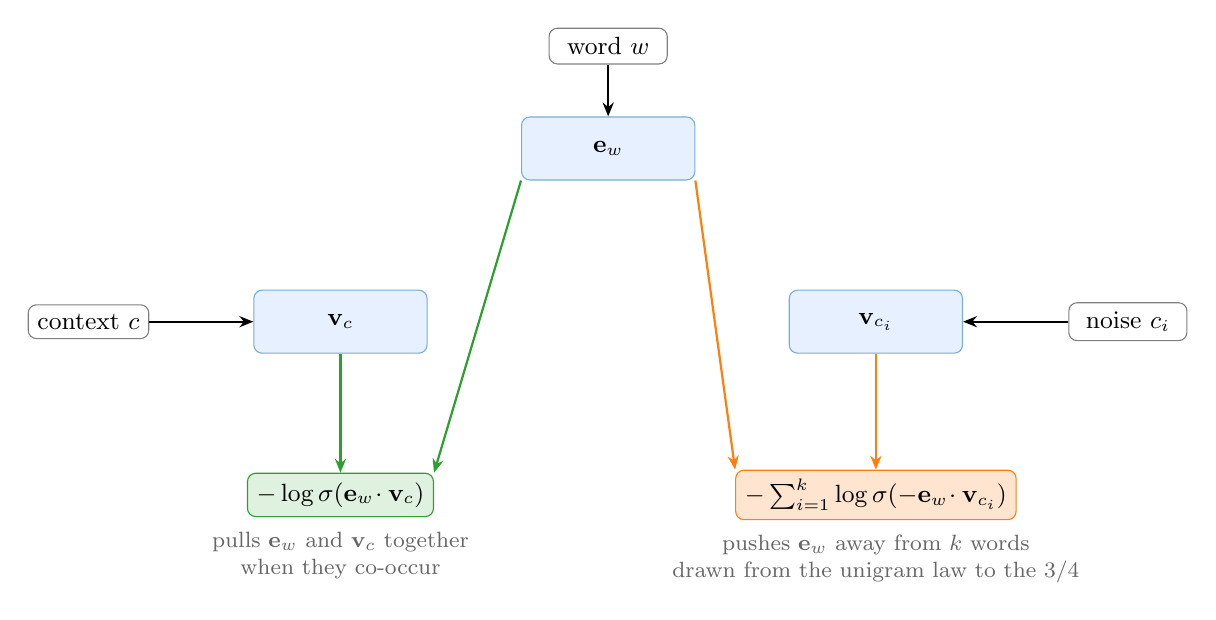
\begin{tikzpicture}[font=\small]
  \node[draw=aux, rounded corners=3pt, minimum width=1.5cm] (w) at (0,1.3) {word $w$};
  \node[encoder, minimum width=2.2cm] (e) at (0,0) {$\mathbf{e}_w$};
  \draw[flow] (w) -- (e);
  \node[draw=aux, rounded corners=3pt, minimum width=1.5cm] (c) at (-6.6,-2.2) {context $c$};
  \node[encoder, minimum width=2.2cm] (v) at (-3.4,-2.2) {$\mathbf{v}_c$};
  \draw[flow] (c) -- (v);
  \node[draw=aux, rounded corners=3pt, minimum width=1.5cm] (n) at (6.6,-2.2) {noise $c_i$};
  \node[encoder, minimum width=2.2cm] (vn) at (3.4,-2.2) {$\mathbf{v}_{c_i}$};
  \draw[flow] (n) -- (vn);
  \node[draw=msg, fill=msg!15, rounded corners=3pt] (pos) at (-3.4,-4.4) {$-\log\sigma(\mathbf{e}_w\!\cdot \mathbf{v}_c)$};
  \node[draw=highlight, fill=highlight!20, rounded corners=3pt] (neg) at (3.4,-4.4) {$-\sum_{i=1}^{k}\log\sigma(-\mathbf{e}_w\!\cdot \mathbf{v}_{c_i})$};
  \draw[flow, msg] (e.south west) -- (pos.north east);
  \draw[flow, msg] (v) -- (pos);
  \draw[flow, highlight] (e.south east) -- (neg.north west);
  \draw[flow, highlight] (vn) -- (neg);
  \node[annotation, align=center, below=2pt of pos] {pulls $\mathbf{e}_w$ and $\mathbf{v}_c$ together\\when they co-occur};
  \node[annotation, align=center, below=2pt of neg] {pushes $\mathbf{e}_w$ away from $k$ words\\drawn from the unigram law to the $3/4$};
\end{tikzpicture}
\end{document}
